\chapter{Background} \label{b} \label{chap:b}
This section is an overview of techniques that influence the design choices of our monadic language for parallel computation. First of all, we give an overview of techniques applied in the high-level parallel programming framework: arrows (\secref{b:arrows}) and recursion schemes (\secref{b:rs}). We then introduce several techniques for message-passing concurrency: multiparty session types (\secref{b:mpst}) and monadic languages for concurrency (\secref{b:mo}). In the end, we introduce free monads (\secref{b:fm}), a technique valuable in implementing embedded domain-specific languages (EDSL).

\section{Arrows} \label{b:arrows}
Arrow is a general interface to describe computation. It can ease the process of writing structured code suitable for parallelizing. It also demonstrates a common feature of the frameworks: parallelizability is empowered by underlying implicit but precise data-flow. On the other hand, converting to low-level message-passing code, which requires programmers to define communication using message-passing function and primitives, makes the data-flow explicit.
\subsection{Definition}
\coref{b:ar:c1} shows the Arrow definition in Haskell. Intuitively, an arrow type \hask{y a b}(that is, the application of the parameterised type \hask{y} to the two parameter types \hask{b} and \hask{c}) can be regarded as a computation with input of type \hask{b} and output of type \hask{b}\cite{hughesGeneralisingMonadsArrows2000}. Visually, arrows are like pipelines (shown in \figref{b:ar:p1}). In Haskell, an arrow \hask{y} is a type that implements the following interface (type classes in Haskell are roughly interfaces). \hask{arr} converts an arbitrary function into an arrow. \hask{>>>} sequences two arrows (illustrated in \figref{b:ar:seq}). Taking two input,  \hask{first} apply the arrow to the first input while keeping the second untouched (\figref{b:ar:first}). Conversely, \hask{second} modifies the second input and keeps the first one unchanged. \hask{***} applies two arrows to two input side by side (\figref{b:ar:par}). \hask{&&&} takes one input and applies two separate arrows to the input and its duplications (\figref{b:ar:dup}).

The simplest instance of arrow class is the function type (shown in \coref{b:ar:c2}). It is worth noticing that only \hask{arr} and \hask{***} need to be implemented. The rest of functions in the arrow type class can be defined in terms of the two functions. For example, \mintinline{text}{f &&& g = (f *** g) . arr (\b -> (b, b))} and \mintinline{text}{first = (*** id)}
\begin{listing}[ht]
  % \inputminted{haskell}{background/ar-def.hs}
  \begin{minted}{haskell}
    class Arrow y where 
      arr :: (a -> b) -> y a b
      first :: y a b -> y (a, c) (b, c)
      second :: y a b -> y (c, a) (c, b)
      (***) :: y a c -> y b d -> y (a, b) (c, d)
      (&&&) :: y a b -> y a c -> y a (b, c)
  \end{minted}
  \caption{Arrow class in Haskell}
  % \ccaption{Arrow class in Haskell}{
    % \begin{itemize}
      % \item[\cref{ar-def:1}] Types of arrow functions 
    % \end{itemize}
  % }
  \label{b:ar:c1}
\end{listing}
\begin{listing}[ht]
  % \inputminted{haskell}{background/ar-func.hs}
  \begin{minted}{haskell}
    instance Arrow (->) where
      arr f = f
      (***) f g ~(x,y) = (f x, g y)
  \end{minted}
  \caption{$(\rightarrow)$ instance of Arrow class}
  \label{b:ar:c2}
\end{listing}
\begin{figure*}
  \centering
  \begin{subfigure}[b]{0.475\textwidth}
      \centering
      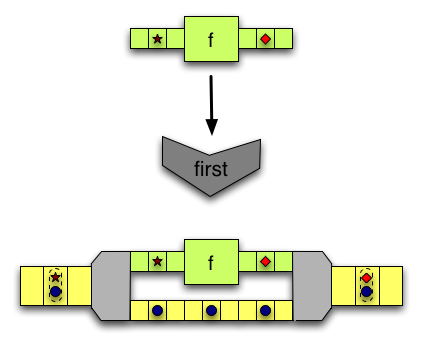
\includegraphics[width=\textwidth]{background/image/ArrowsConveyors_first2.png}
      \caption{\hask{first}}
      \label{b:ar:first}
  \end{subfigure}
  \hfill
  \begin{subfigure}[b]{0.475\textwidth}  
      \centering 
      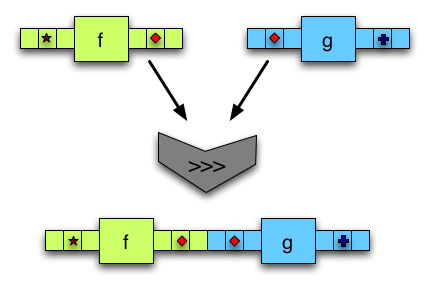
\includegraphics[width=\textwidth]{background/image/ArrowsConveyors_bind2.png}
      \caption{\hask{>>>}}
      \label{b:ar:seq}
  \end{subfigure}
  \vskip\baselineskip
  \begin{subfigure}[b]{0.475\textwidth}   
      \centering 
      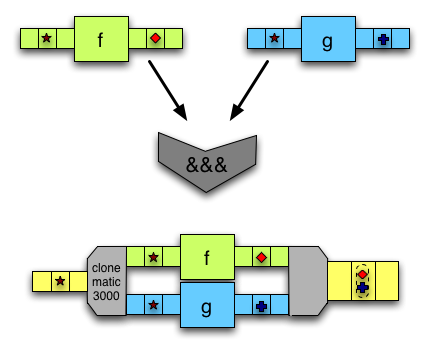
\includegraphics[width=\textwidth]{background/image/ArrowsConveyors_ampersand2.png}
      \caption{\hask{&&&}}
      \label{b:ar:dup}
  \end{subfigure}
  \quad
  \begin{subfigure}[b]{0.475\textwidth}   
      \centering 
      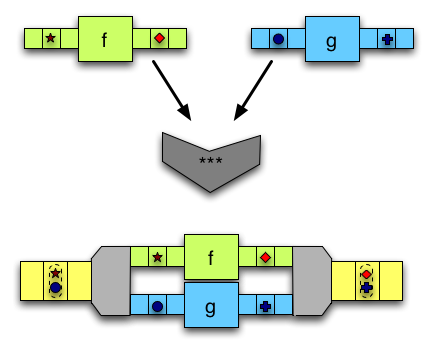
\includegraphics[width=\textwidth]{background/image/ArrowsConveyors_star2.png}
      \caption{\hask{***}}
      \label{b:ar:par}
  \end{subfigure}
  \caption
  {\small The visual representations of arrow combinators\cite{HaskellUnderstandingArrows}}
  \label{b:ar:p1}
\end{figure*}
\subsection{Example: Calculate the mean}
Consider the function to calculate the mean from a list of floating point numbers, we present the implementation using arrows compared with a point-free Haskell definition. Implementation using arrows can be regarded as point-free programming. Point-free programming is programming paradigm where function definitions only involve combinators and function composition without mentioning variables \cite{TacitProgramming2019}. 

\begin{minted}{haskell}
mean :: [Float] -> Float
mean xs = sum xs / (fromIntegral . length) xs

mean' :: [Float] -> Float
mean' = (sum &&& (length >>> fromIntegral)) >>> uncurry (/)
\end{minted}
The arrows implementation can be visualised in \figref{b:ar:p2}.
\begin{figure}[!ht]
  \centering
  % \includegraphics[width=8cm]{example-image} 
  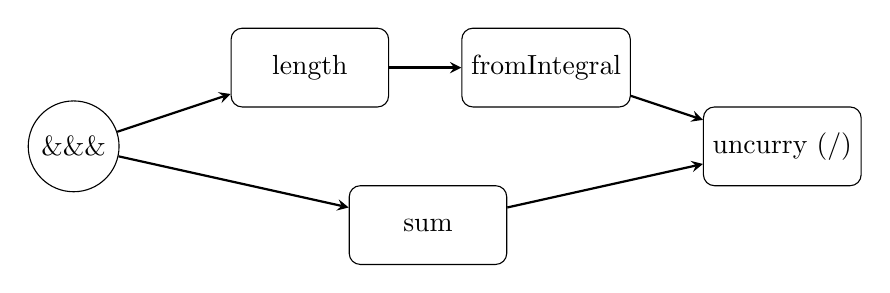
\begin{tikzpicture}[xscale=1.5]
    \tikzstyle{proc} = [rectangle, rounded corners, minimum width=2cm, minimum height=1cm,text centered, draw=black] 
    \tikzstyle{proc1} = [circle,  minimum width=1cm, minimum height=1cm,text centered, draw=black] 
    \tikzstyle{arrow} = [thick,->,>=stealth]
    \node (a) [proc1] at (0, 0) {\&\&\&};
    \node (b) [proc] at (2, 1) {length};
    \node (c) [proc] at (4, 1) {fromIntegral};
    \node (d) [proc] at (6, 0) {uncurry (/)};
    \node (e) [proc] at (3, -1) {sum};
    \draw[arrow] (a) to (b);
    \draw[arrow] (b) to (c);
    \draw[arrow] (c) to (d);
    \draw[arrow] (a) to (e);
    \draw[arrow] (e) to (d);
  \end{tikzpicture}
  \caption{Visualization of mean'}\label{b:ar:p2}
\end{figure}
\begin{minted}{haskell}
mean'' :: [Float] -> Float
mean'' = liftM2 (/) sum (fromIntegral . length)
\end{minted}
The above code snippet is the more traditional approach form of point-free mean function in Haskell. Arrows are not the only way to form point-free programs. We can argue this form of point-free function is more difficult to understand compared to arrows because it involves knowledge of monads (\hask{liftM2}) and does not map to the intuitive data-flow.

The simple example demonstrates that arrows combinators make writing point-free programs easier. Arrows unite the implementation of algorithm and data-flow in the algorithm. 

\subsection{Application in parallel computation}
From the previous example, the data flow of programs written using arrow combinators can be easily visualized (shown in \figref{b:ar:p1}). It is intuitive to recognize that the clean separation between the flow of data and actual computation will be useful in generating parallel code. Indeed, arrow describes data flow implicitly, and it is an example of the so-called algebraic pattern. Many works has been done to generate parallel code from algebraic patterns \cite{braunArrowsParallelComputation2018, elliottGenericFunctionalParallel2017b, AlgebraicMultipartyProtocol}. In particular, details of \cite{AlgebraicMultipartyProtocol} are introduced in \charef{chap:alg}.

We will use some figures to explain the idea behind arrows as a framework for parallel computation. For example, as shown in the \figref{b:ar:p3}, \hask{f *** g} means computations of \hask{f} and \hask{g} happen in parallel. \figref{b:ar:p4} shows that it can be used to implement parallel map in terms of arrows, taking an arrow computation \hask{arr a b} and returning a list of computation in parallel (\hask{arr [a] [b]}). 
\begin{figure*}[ht]
\begin{subfigure}[b]{0.475\textwidth}
  \centering
  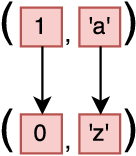
\includegraphics[width=\textwidth/3]{background/image/pareval2.png}
  \caption{Visualization of parallel \hask{***}\cite{braunArrowsParallelComputation2018}}
  \label{b:ar:p3}
\end{subfigure}
\hfill
\begin{subfigure}[b]{0.475\textwidth}
  \centering
  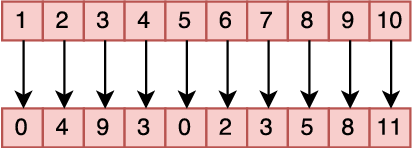
\includegraphics[width=\textwidth]{background/image/parevaln.png}
  \caption{Visualization of parMap \cite{braunArrowsParallelComputation2018}}
  \label{b:ar:p4}
\end{subfigure}
\end{figure*}
\section{Recursion Schemes} \label{b:rs}
Recursion schemes are patterns for expressing recursive functions. In particular, they are high order function abstracting common patterns of recursion.
\subsection{Definition}
We will introduce three typical recursion schemes: catamorphisms representing folds, anamorphisms representing unfolds and hylomorphisms representing divide-and-con\-quer algorithms (seen in \coref{p:pal:c3}). Recursion schemes express recursion with the help of data structures that mirror the control structure of the recursion.

\begin{listing}[ht]
\begin{minted}{haskell}
newtype Fix f = Fix { unfix :: f (Fix f) }

data TreeF a =
    Node a a
  | Leaf int
  | Empty
  deriving Functor

type Tree = Fix TreeF
\end{minted}
\caption{Definition of fix point of data structures} \label{p:pal:c2}
\end{listing}

Anamorphisms takes a function from a to f a (called the co-algebra) and a value a and return the Fix f. Used Tree as an example, anamorphisms takes a single value with type a and applies the co-algebra to the value. It continues to apply itself to the branches of the TreeF recursively and finally expands a single value to a complete tree. Intuitively, anamorphism unfolds a single value to a complicated data structure top-down.

Catamorphisms are the reverse of anamorphisms, folding a data structure to a single value bottom-up. It takes a function from f a to a (called the algebra) and Fix f to fold and return a single value a. Catamorphisms and anamorphisms describe the process globally (from a to Fix f and from Fix f to a) while co-algebra and algebra capture what happened locally. The elegant part is while co-algebra and algebra do not involve with any recursion data structure (TreeF is not recursive), catamorphisms consumes recursive data structure while anamorphism builds them.

Hylomorphisms applies anamorphism followed by catamorphisms. It is the most common pattern to use. We will use an example to illustrate its usefulness. It can be thought of as an abstract divide and conquer algorithm.
\begin{listing}[ht]
\begin{minted}{haskell}
ana :: Functor f => (a -> f a) -> a -> Fix f
ana coalg = Fix . fmap (ana coalg) . coalg

cata :: Functor f => (f a -> a) -> Fix f -> a
cata alg = alg . fmap (cata alg) . unfix

hylo :: (f b -> b) -> (a -> f a) -> b -> a 
hylo g f = f . fmap (hylo f g) . g
\end{minted}
\caption{Recursion schemes in haskell} \label{p:pal:c3}
\end{listing}

\subsection{Example: Merge sort} \label{b:rs:ex}
We can write merge sort recursively. First of all, we split the list in half and then apply the merge sort recursively to both parts and finally we merge two lists into a single list. 

To write merge sort in terms of recursion scheme, we need to define the recursive structure to represent the control structure. By the definition of merge sort, this structure must have a case with two branches, a base case representing a singleton list and a base case representing an empty list hence this structure is the TreeF we defined above. Splitting a list is a co-algebra while merging is a algebra. We use hylomorphisms to combine them hence getting a sorted list (seen in \coref{p:pal:c4}).
\begin{listing}[ht]
\inputminted{haskell}{project/pal-ms.hs}
\caption{Merge sort using hylomorphisms} \label{p:pal:c4}
\end{listing}
\section{Multiparty session types} \label{b:mpst}
In complicated distributed systems, participants agree on a protocol, specifying the type and direction of data exchanged. Multiparty session types are a branch of behavioral types specifically targeted at describing protocols in distributed systems based on asynchronous communication \cite{coppoGentleIntroductionMultiparty2015}. They are a type formalism used to model communication-based programming by codifying the structure of the communication. The evolution of computing from the era of data processing to the era of communication witnessed the growth and significance of the theory of session types.

The theory of multiparty session types contains three main elements. Global types (seen in \secref{b:mpst:st}), local (session) types and processes. Processes are the concrete descriptions of the behavior of the peers involved in the distributed system \cite{coppoGentleIntroductionMultiparty2015} using a formal language. The most used and the original language is $\pi$-calculus \cite{milnerCalculusMobileProcesses1992}. The coming sections are an intuitive introduction of session types by examples.
% TODO: Add descriptions about the MPST 1. describes explicit dataflow 2. so it can be used as the high-level programming languages to generate parallel code 3. in \secref{b:mpst:app}.
\subsection{Global types and local types} \label{b:mpst:st}
A global type is at the most abstract level, describing a communication protocol from a neutral viewpoint between two or more participants\cite{coppoGentleIntroductionMultiparty2015}. The syntax of global types is shown in \figref{b:mpst:gt} and an example of global types is shown in \figref{b:mpst:gtex}.

Local types or session types characterise the same communication protocol as the global type, but from the viewpoint of each peer \cite{coppoGentleIntroductionMultiparty2015}. Each process is typed by a local type. The syntax of local types is shown in \figref{b:mpst:lt} and an example of local type is shown in \figref{b:mpst:ltex}. 

The relationship between global types and local types are established by the projection operator (seen in the \secref{b:mpst:proj}), and a type system performs syntactic checks, ensuring that processes are typed by their corresponding local types. Hence, at the compile time, three important properties follow \cite{coppoGentleIntroductionMultiparty2015}. 
\begin{itemize}
  \item \textbf{communication safety}: Mismatches between the types of sent and expected messages, despite the same communication channel is used for exchanging messages of different types, do not exist \cite{coppoGentleIntroductionMultiparty2015}. 
  \item \textbf{protocol fidelity}: The interactions that occur are accounted for by the global type and therefore are allowed by the protocol \cite{coppoGentleIntroductionMultiparty2015}.
  \item \textbf{progress}: Every message sent is eventually received, and every process waiting for a message eventually receives one \cite{coppoGentleIntroductionMultiparty2015}.
\end{itemize}
We will learn that these properties are valuable not only in the distributed system but also in the domain of parallel computing in \secref{b:mpst:app}.
% In the theory of multiparty session types, the whole distributed system is described by global types representing the communication protocols from a global viewpoint.  Each process is typed by local types which characterise the same communication protocols as global types but from a perspective of individual participants \cite{coppoGentleIntroductionMultiparty2015}.
\begin{figure}[ht]
\centering
\begin{grammar}{G\Coloneqq}{Global types}
  p \rightarrow q : \langle S \rangle.G & Value exchange \\
  p \rightarrow q : \langle T \rangle.G & Channel exchange \\
  p \rightarrow q : \{ l_i : G_i \}_{i \in I} & Bracnhing \\
  \mu \mathbf{t}.G  \mid \mathbf{t} \mid \text{end} & Recursion/End
\end{grammar}
\caption{Global types} \label{b:mpst:gt}
\end{figure}
\begin{figure}[ht]
\begin{grammar}{S\Coloneqq}{Sorts}
  \text{bool} \mid \text{nat} \mid \text{string} \\
  \dots\\
\end{grammar}
\hfill
\begin{grammar}{T\Coloneqq}{Session types/local types}
  ! \langle p, S \rangle . T & Send value\\
  ! \langle p, T \rangle . T & Send channel\\
  ? ( p, T ) . T & Channel Receive\\
  ? ( p, S ) . T & Sorts Receive\\
  \oplus \langle p, \{ l_i : T_i \}_{i \in I} \rangle & Selection \\
  \&(p, \{l_i : T_i \}_{i \in I}) & Bracnhing \\
  \mu \mathbf{t}.T  \mid \mathbf{t} \mid \text{end} & Recursion/End
\end{grammar}
\caption{Session types/local types} \label{b:mpst:lt}
\end{figure}
\begin{figure}[ht]
  \begin{minipage}{0.45\textwidth}
    \begin{enumerate}
      \item Customer(0) sends an order number to Agency(1), and the Agency sends back a quote to the customer.
      \item If Customer is happy with the price, then Customer selects accept option and notifies Agency.
      \item If Customer thinks the price is too high, then Customer terminate the trade by selecting reject.
      \item If accept is selected, the Agency notifies both Customer and Agency2(2). 
      \item Customer sends an address to Agency2 and Agency2 sends back a delivery date.
    \end{enumerate}
  \end{minipage}
  \hfill
  \begin{minipage}{0.45\textwidth}
    \begin{align*}
      G = \\
      & 0 \rightarrow 1: && \langle \text{string} \rangle .\\
      & 1 \rightarrow 0: && \langle \text{int} \rangle .\\
      & 0 \rightarrow 1: \{ && \text{accept}: \\
      & && 1 \rightarrow \{ 0, 2 \}: \langle \text{string} \rangle . \\
      & &&  0 \rightarrow 2: \langle \text{string} \rangle .\\
      & &&  2 \rightarrow 0: \langle \text{int} \rangle . \text{end}, \\
      & && \text{reject}: \text{end} \} \\
    \end{align*}
  \end{minipage}
  \caption{An example of a protocol described by global types G}
  \label{b:mpst:gtex}
\end{figure}
\begin{figure}[ht]
  \begin{minipage}{0.45\textwidth}
    \begin{align*}
      S \triangleq \mu t.(\&\{ & \text{balance}: ![\text{nat}];t, \\
        & \text{deposit}: ?[\text{nat}];![\text{nat}];t, \\
        & \text{exit}: \text{end}\}) \\
    \end{align*}
  \end{minipage}
  \hfill
  \begin{minipage}{0.45\textwidth}
    \begin{align*}
      C \triangleq \oplus \{ &\text{balance}: ?[\text{nat}];\text{end}, \\
                             &\text{deposit}: ![\text{nat}];?[\text{nat}];\text{end} \} 
    \end{align*}
  \end{minipage}
  \caption{Session types of client and server end point of a ATM service}
  \label{b:mpst:ltex}
\end{figure}
\subsubsection{Projection between global types and local types} \label{b:mpst:proj}
Projection is the formalization of the relationship between global and local types. It is an operation extracting the local type of each peer from the global type \cite{coppoGentleIntroductionMultiparty2015}. The definition of projection is shown in \figref{b:mpst:pdef}.

As an example, a projection of global type in \figref{b:mpst:gtex} is
$$
  G \upharpoonright 0 = !\langle 1, \text{string} \rangle;?(1, \text{string});\&(1, \{ \text{accept}: ?(1, \text{string});!\langle 2, \text{string} \rangle;?(2, \text{int}), 
  \text{reject}: \text{end} \})
$$  
\begin{figure}[H]
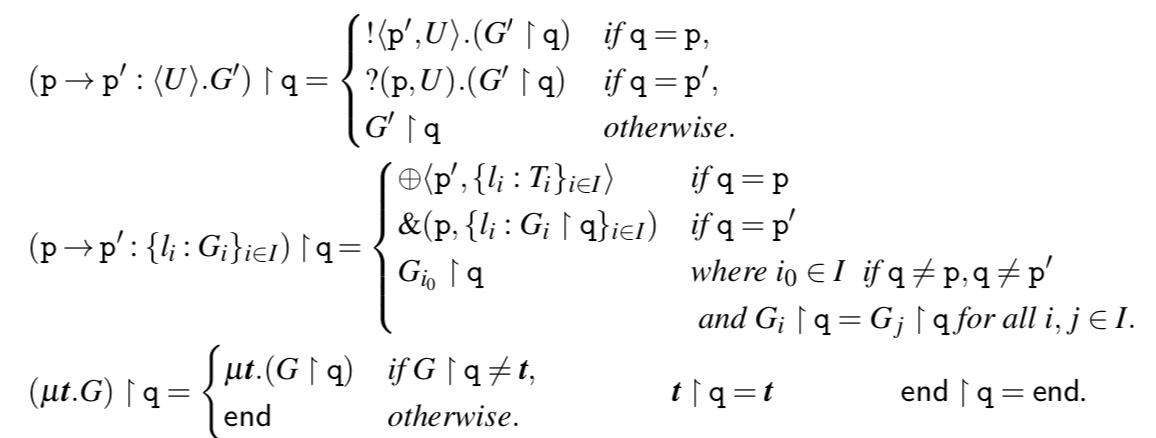
\includegraphics[width=\textwidth]{background/image/proj-def.png}
\caption{The definition of projection of a global type G onto a participants q\cite{coppoGentleIntroductionMultiparty2015}}
\label{b:mpst:pdef}
\end{figure}
\subsubsection{Duality of session types}
In binary session types where all protocals are pairwise, duality formalises the relationship between the types of opposite endpoints. For a type $T$, its dual or co type, written $\bar{T}$ is defined inductively as in \figref{b:mpst:dualdef}.
\begin{figure}[H]
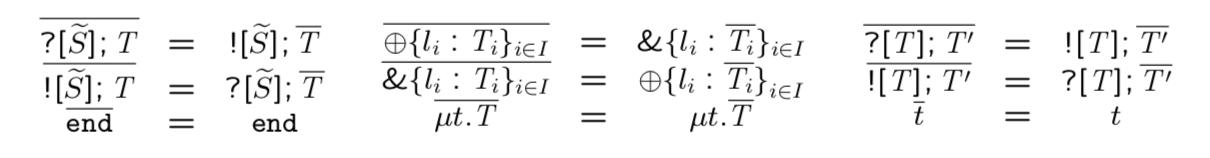
\includegraphics[width=\textwidth]{background/image/dual-def.png}
\caption{Inductive definition of duality}
\label{b:mpst:dualdef}
\end{figure}

Duality is essential for checking type compatibility. Compatible types mean that each common channel $k$ is associated with complementary behavior: this ensures that the interactions on $k$ run without errors. 

In order to apply duality into multiparty session types in which more than two participants are allowed, the partial projection operation (seen in \cite{coppoGentleIntroductionMultiparty2015}) from multiparty session type to binary session type was introduced to allow reusing the definition of duality after applying the partial projection.
% \begin{table}[H]
% \caption{The pa}
% \label{b:mpst:partproj}
% \end{table}
% \begin{table}[ht]
% \begin{align*}
% \end{align*}
% \caption{Inductive definition of duality} \label{b:mpst:dual}
% \end{table}
% \subsection{Example: arithmetic server}
\subsection{Applications in parallel computing} \label{b:mpst:app}
Multiparty session types not only have rich applications in distributed systems but also value in the domain of parallel computation. 

Existing work\cite{ngProtocolsDefault2015} has shown how to generate Message Passing Interface (MPI) \cite{MessagePassingInterface} programs using session types. Users describe the communication topology as a skeleton using a protocol language, which is type checked by session types. After that, an MPI program is generated by merging the skeleton and user-provided kernels for each peer. The parallel code obtained in this way is guaranteed to be deadlock-free and progressing. 

\section{Message passing concurrency} \label{b:mo}
This section introduces some interfaces for message passing concurrency from the primitive case: channel to more advanced one: monad for message passing concurrency.

For simplicity, they are represented in Haskell, but in general, most languages can implement similar interfaces. 
\subsection{Primitives for message-passing concurrency} \label{b:mo:mpc}
In \secref{b:mpst}, channels are bi-directional and used for communication between two parties. In Haskell, channel primitives are represented in \coref{b:mo:c1}. However, just using these primitives cannot guarantee progress or communication safety. For example, a program that has one thread writing channel once combined with another thread reading channel twice is type-correct but will cause deadlock. Many kinds of research to encode MPST using Haskell's type system are presented in \cite{orchardSessionTypesLinearity2017} so that an (MPST) type-correct Haskell program assures progress, communication safety and session fidelity.
\begin{listing}[ht]
  \inputminted{haskell}{background/mo-chan.hs}
  \caption{Channel primitives in Haskell}
  \label{b:mo:c1}
\end{listing}
\subsection{Concurrency Monads}
The work done by \cite{claessenPoorManConcurrency1999} constructs a monad to express concurrent computation. The definition is in \coref{b:mo:def}. \hask{Action} is the algebraic datatype representing basic concurrency primitives. \hask{Atom}, the atomic unit of computation, is a computation (wrapped in the \hask{IO} monad) followed by an action. \hask{Fork} is two parallel action. \hask{Stop} is the termination of an action. type \hask{C} is a special case of the continuation monad. The continuation monad is an encapsulation of computations in continuation-passing style (CPS)\footnote{In continuation-passing style function result is not returned, but instead is passed to another function, received as a parameter (continuation)\cite{ControlMonadCont}}. SO \hask{C a} is a CPS computation that produces an intermediate result of type \hask{a} within a CPS computation whose final result type is \hask{Action}. With the help of the monad \hask{C}, sequencing and composing actions can use monadic bind.
\begin{listing}[ht]
  \begin{minted}{haskell}
data Action =
    Atom (IO Action)
  | Fork Action Action
  | Stop

newtype C a = C { runC :: (a -> Action) -> Action }
    
instance Monad C where
    (>>=) :: C a -> (a -> C b) -> C b
    m >>= f  = C $ \k -> runC m (\v -> runC (f v) k)
    return :: a -> C a
    return x = C $ \k -> k x
  \end{minted}
  \caption{The definition of concurrency monad}
  \label{b:mo:def}
\end{listing}


The idea is using continuation to represent the "future" so that computation can pause and resume as well as expressing sequential computation. Atom wraps the actual computation and Fork is responsible for spawning threads. In addition, in order to write programs in a monadic way easier, some helper functions are defined (shown in \coref{b:mo:helper}). \hask{atom} lifts an IO computation to \hask{C}. And \hask{fork} takes a computation in \hask{C} and return a \hask{C} which involves the \hask{Fork} action. Given a \hask{C a}, \hask{action} gives the result of running the CPS computation. We use \hask{\_. Stop} to represent the final continuation (\hask{Stop} action is the last action). 
\begin{listing}[ht]
\begin{minted}{haskell}
atom :: IO a -> C a
atom m = C $ \k -> Atom $ do
    r <- m
    return $ k r

fork :: C () -> C ()
fork m = C $ \k -> Fork (runC m (const Stop)) (k ())

action :: C a -> Action
action m = m (\_. Stop)
\end{minted}
\caption{Helper functions}
\label{b:mo:helper}
\end{listing}
An example of programme written in the concurrency monad is shown below.
\begin{code}
  \begin{minted}{haskell}
example :: C ()
example = do 
  atom $ putStrLn "Hello" 
  name <- atom getLine 
  fork $ atom $ putStrLn "World"
  atom $ putStrLn name
  \end{minted}
\end{code}
We can easily define a round-robin scheduler for programs in this monad. We can regard a list of action as a queue of threads that are running concurrently. \hask{schedule} will pattern match on the head of the list. If it is \hask{Atom} then the scheduler will run the computation (seen \hask{a <- ioa} at \cref{mo-cm:1}) and pause its remaining computation and put it at the end of the thread queue (seen at \cref{mo-cm:2}). If it is \hask{Fork} then the scheduler will spawn the thread and put the new thread and the current thread to the bottom of the queue (seen at \cref{mo-cm:3}). Finally, If it is \hask{Stop} then it means this thread has finished, and the scheduler will resume with the rest of threads in the queue. For example, to run the above example, we call \hask{schedule [action example]}.
\begin{code}
  \begin{minted}{haskell}
schedule :: [Action] -> IO () 
schedule [] = return ()
schedule (a:as) = sched as a

sched :: [Action] -> Action -> IO ()
sched as (Atom ioa) = do
    a <- ioa #\clabel{mo-cm:1}#
    schedule $ as ++ [a] #\clabel{mo-cm:2}#
sched as (Fork a1 a2) = schedule $ as ++ [a2, a1] #\clabel{mo-cm:3}#
sched as Stop = schedule as
  \end{minted}
\end{code}

The concurrency monad can be extended to support many features. For example, work done by \cite{marlowMonadDeterministicParallelism2011} modifies the definition of Action as well as implements a work-stealing parallel scheduler (seen in \coref{b:mo:c3}) to build a monad for parallel computation. 

Besides, extending the concurrency monad to monad for message-passing concurrency can be done by adding channel primitives like newChan, writeChan and readChan into the Action. Since channel primitives are possible to represent in this monad, we naturally think of its prospect in connecting with MPST (will be discussed in \secref{spar:sec:session-typing})
\begin{listing}[ht]
  % \inputminted{haskell}{background/mo-par.hs}
  \begin{minted}{haskell}
newtype IVar a = IVar (IORef (IVarContents a)) #\clabel{po:ivar}#
data IVarContents a = Full a | Blocked [a -> Action.]
    
data Action .=
    Fork Action Action
  | Stop
  | forall a . Get (IVar a) (a -> Action) #\clabel{po:get}#
  | forall a . Put (IVar a) a Action #\clabel{po:put}#
  | forall a . New (IVar a -> Action)
  \end{minted}
  \ccaption{Par Monad}{
    \begin{itemize}
      \item[\cref{po:ivar}] Parent threads and child threads communicate data via IVar
      \item[\cref{po:get}] Get operation blocks when the underlying IVarContents is Blocked  
      \item[\cref{po:put}] Put operation updates the underlying IVarContetns to Full with the result a and resume the list of blocking threads by applying a to the continuation.
    \end{itemize}
  }
  \label{b:mo:c3}
\end{listing}

We draw inspiration from this monad to design our intermediate language.
\section{Free monad} \label{b:fm}
Free monad \cite{FreeMonadNLab} is a concept from category theory. Intuitively, a free monad as a programming abstraction is a technique for implementing EDSLs, where a functor represents basic actions of the EDSL and the free monad of this Functor provides a way to sequence and compose actions. Speaking of the advantages, we are particularly interested in its benefits in flexible interpretations which will be illustrated by an example (\secref{b:fm:e}) and discussed further (\secref{b:fm:a}).
\subsection{Definition}
In practice, a free monad in Haskell can be defined as an algebraic data type(ADT) (shown in \coref{b:fm:c1}). \hask{Free f} is the monad produced given a functor \hask{f}. \hask{Free} has two type constructors: \hask{Pure} and \hask{Free}. \hask{Monad (Free f)} is the Haskell implementation of the Monad interface for \hask{Free f}. Many useful helper functions are derived from the simple definition of the free monad (shown in \coref{b:fm:c2}). \hask{liftF} lift the functor to its free monad representations. \hask{freeM} maps a natural transformation of functor (\hask{f a -> g a}) to the natural transformation of their free monad versions. Given \hask{m} is a monad, \hask{freeM} is a special case of interpreting \hask{Free m a}: to the \hask{m} monad itself. Finally, \hask{interpret} shows the power of free monad. We can interpret the free monad version of a functor \hask{f} to any monad \hask{m} given a natural transformation from \hask{f} to \hask{m}.
\begin{listing}[ht]
  \inputminted{haskell}{background/fm-construction.hs}
  \caption{Free monad in Haskell}
  \label{b:fm:c1}
\end{listing}
\begin{listing}[ht]
  \inputminted{haskell}{background/fm-helper.hs}
  \caption{Helper functions based on free monad}
  \label{b:fm:c2}
\end{listing}
\subsection{Example} \label{b:fm:e}

Free monad is useful in interpreting an abstract syntax tree (AST). In order to apply free monad to a given AST, we can follow a routine \cite{contributorsCatsFreeMonadsa}.

\begin{enumerate}
  \item Create an AST, usually represented as an ADT
  \item Implement functor for the ADT
  \item Create helper constructors to Free ADT for each type constructor in ADT by liftF 
  \item Write a monadic program using helper constructors. It is essentially a program written in EDSL operations.
  \item Build interpreters for Free ADT by interpreting
  \item Interpret the program by the interpreter.
\end{enumerate}
We will demonstrate the above procedure by a made-up example. We would like to build a simple EDSL for getting customers' name and greeting customers. First of all, we build a functor \hask{GreetingF} to represent the basic operations: getting the name and greeting. Then we wrap the functor with \hask{Free} constructor so that a program written in our EDSL can be regarded as a Haskell expression with type \hask{Free GreetingF a}.
\begin{code}
\begin{minted}{haskell}
data GreetingF next
  = Getname (String -> next)
  | Greet String next
  deriving Functor

type Greeting = Free GreetingF
\end{minted}
% \caption[.]{
%   \begin{minipage}{\linewidth}
%     Par monad
%     \begin{itemize}
%       \item[\cref{mylin2} :] hello 
%       \item[\cref{mylin2} :] hello 
%     \end{itemize}
%  \end{minipage}
%  }
\end{code}
Then we create helper functions of Greeting using liftF.
\begin{minted}{haskell}
getName = liftF $ Getname id
greet str = liftF $ Greet str ()
\end{minted}
Then we can write a simple program using operations provided by Greeting.
\begin{minted}{haskell}
exampleProgram :: Greeting ()
exampleProgram = do
    a <- getName
    greet a
    b <- getName
    greet b
\end{minted}
Then we can easily implement an interpreter for the example program
\begin{minted}{haskell}
goodMorningInterpreter :: Greeting a -> IO a
goodMorningInterpreter = interpret helper
    where
        helper (Getname next) = 
          fmap next getLine
        helper (Greet str next) =
          putStrLn ("Good morning " ++ str) >> return next  
\end{minted} 
Finally, execute the program.
\begin{minted}{bash}
ghci:> goodMorningInterpreter exampleProgram
Tom
Good morning Tom
Mary
Good morning Mary
\end{minted}
% \begin{listing}
%   \inputminted{haskell}{background/fm-example.hs}
%   \caption{An example of free moand}
%   \label{b:fm:c3}
% \end{code}

\subsection{Applications} \label{b:fm:a}
As illustrated by the example (\secref{b:fm:e}), free monad decouple the abstract syntax tree of domain specific language (EDSL) and the interpreter. Interpreters with different purposes can be implemented without changing the syntax.

In the project, we apply free monad to the intermediate language so not only we make the languages monadic for free but also benefits from decoupling the interpreter and the syntax to implement different interpreters, e.g. Simulator, code generators to different platforms easily.